\documentclass[11.5pt, a4paper]{article}

\usepackage[english]{babel}
\usepackage[export]{adjustbox}
\usepackage{amsmath}
\usepackage{graphicx}
\usepackage[colorinlistoftodos]{todonotes}

\usepackage{geometry}


\fboxsep=5mm%padding thickness

\usepackage{tabularx, booktabs}
\usepackage{hologo}
\usepackage{multicol}
\usepackage{hyperref}
\usepackage{titlesec}
% DOCUMENT LAYOUT


 \geometry{
 a4paper,
 left=40mm,
 right=40mm,
 top=30mm,
 bottom=20mm,
 }



\title{\huge Web Crawler}
\author{
Saurabh Mathur\\
\texttt{14BIT0180}
\and
Tushar Bhatia\\
\texttt{14BIT0163}
}


\usepackage[final,factor=1100,shrink=10]{microtype}
\linespread{0.95833}

\begin{document}

\maketitle



\section*{Abstract}

A Web crawler is an Internet bot which systematically browses the World Wide Web, typically for the purpose of Web indexing.
The large size and the dynamic nature of the Web makes it necessary to continually
maintain Web based information retrieval systems. Crawlers facilitate this process by following
hyperlinks in Web pages to automatically download new and updated Web pages.
They exploit the graph structure of the Web to move from
page to page.

\section*{Problem Description}

\begin{description}
\item[Input] A list of seed URLs
\item[Output] A set of visited URLs and a graph of the explored network.
\end{description}

\section*{Algorithm}
The Web Crawler will operate as follows: 
\begin{enumerate}
\item Fetch the first HTML page using the seed URL.
\item Parse the HTML document and add all URLs in the document to a list.
\item Fetch each URL from the list.
\item Repeat \texttt{Step 2} and \texttt{Step 3} for each of the URLs in the list.
\end{enumerate}

\begin{figure}[h!]
\centering
      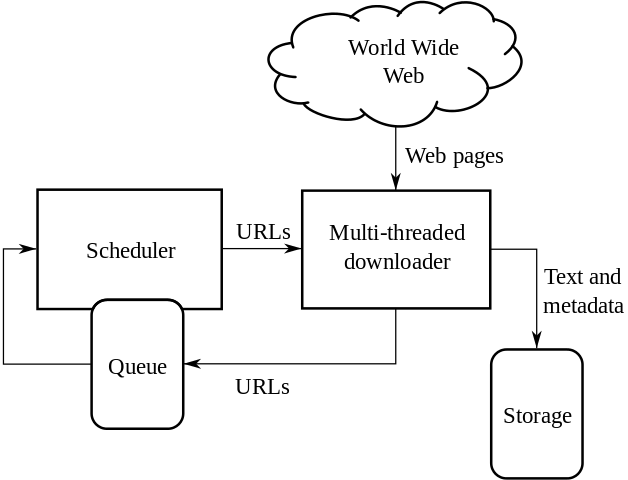
\includegraphics[width=0.6\textwidth, fbox]{WebCrawlerArchitecture.png}
  \caption{Architecture of the Web Crawler}

\end{figure}

\end{document}
